\newcounter{nuserstory}
\newcounter{nusecase}

\newcommand{\userstory}[4]{%
    \refstepcounter{nuserstory}
    \subsection{#1}
    \label{userstory:\thenuserstory}
    \hangindent=40pt
    \textbf{\textit{As a}} #2,\\
    \textbf{\textit{I want to}} #3,\\
    \textbf{\textit{so that}} #4.
}

\chapter{Requirement Analysis}
\label{chap:requirement-analysis}

\section{Stakeholder Analysis}
\label{section:stakeholder-analysis}

\begin{enumerate}[leftmargin=80pt]
    \item \textbf{Animators \& Video Editors:} The primary stakeholders are content creators and 
    video artists who want to protect their work from unauthorized AI training.

\end{enumerate}

\section{User Stories}
\label{section:user-stories}

\userstory{Protecting Video Content from AI Training%
}{digital content creator or video artist%
}{apply adversarial techniques to my videos to prevent AI models from copying my style%
}{I can protect my work from unauthorized AI training while keeping the video unchanged for humans}

\userstory{Ensuring Video Quality for Human Viewers%
}{digital content creator or video artist%
}{apply AI poisoning techniques without affecting the video’s visual quality for humans%
}{my audience can still enjoy my videos without noticeable distortions}

\userstory{Uploading Videos for AI Poisoning%
}{any user who wants to protect their video from AI%
}{upload my video to the system%
}{I can have my content processed and protected}

\userstory{Processing Videos Efficiently%
}{content creator with large video files%
}{have my videos processed quickly without long waiting times%
}{I can protect my videos without delays affecting my workflow}

\userstory{Monitoring Poisoning Progress%
}{user waiting for video processing to complete%
}{see real-time updates on the status of my video poisoning%
}{I know how long the process will take and when my video will be ready}


\section{Use Case Diagram}
\label{section:use-case-diagram}
<TIP: Write a use case diagram for your project here. Refer to an
article “What is a use case diagram?” by Lucidchart for help./>

\section{Use Case Model}
\label{section:use-case-model}
A use case is a detailed description of how a system
interacts with an external entity (such as a user or another system) to
accomplish a specific goal. Use cases provide a high-level view of the
functionality of a system and help in capturing and documenting its
requirements from the perspective of end users.

<TIP: Write use cases for your project here. Make sure to use the
appropriate type of use case for each scenario (brief, casual, and fully-dressed
use case)./>

\section{User Interface Design}
\label{section:user-interface-design}
<TIP: Put the initial design of your application here. You can
showcase a detailed design of a specific page or a sitemap of your application.
See an example below./>

\begin{figure}[h]
    \centering
    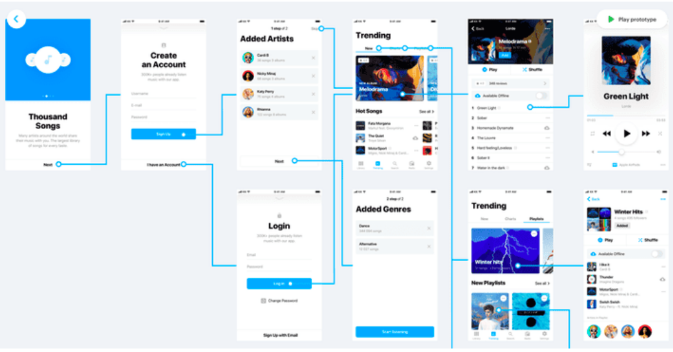
\includegraphics[width=0.8\textwidth]{examples/user-interface-design.png}
    \caption{User Interface Design}
\end{figure}